\documentclass[uplatex]{jsarticle}
\usepackage{amsmath}
\usepackage[dvipdfmx]{graphicx}

\setcounter{tocdepth}{3}
\usepackage{float}
\usepackage{moreverb}
\usepackage{lscape}
%\pagestyle{empty}
%\usepackage{wrapfig}
%\usepackage{url}
%\usepackage{EasyLayout}

\usepackage{ascmac}
%\usepackage{fancybx}

%\pagestyle{myheadings}
\usepackage{hyperref}



\begin{document}


\title{二分法とニュートン法における解の収束の速さについて}
\author{25G1065 塩澤匠生}

%\date{2015年11月13日}
\maketitle


\section{はじめに}
自然界の現象をモデル化するのに方程式が用いられる.
(\ref{eq:omu})式に示されるオームの法則\cite{omu}や(\ref{eq:tou})式に示される等速直線運動\cite{toutyo}については線形の方程式でモデル化できるが
(\ref{eq:dai})式に示されるダイオードの電流電圧特性\cite{daio}や(\ref{eq:jinko})式に示される人口増加モデルなどに用いられるロジスティック方程式\cite{jinko}については線形であるとモデル化できないため
非線形方程式のまま扱う必要がある.

\begin{equation}
V = IR\label{eq:omu}
\end{equation}
\begin{equation}
x = v_0t + x_0\label{eq:tou}
\end{equation}
\begin{equation}
%I = I_S (e^{\frac{V_D}{n V_T}} - 1)\label{eq:dai}
I(V) = I_0 \left[ \exp\left(\frac{eV}{k_B T}\right) - 1 \right]\label{eq:dai}
\end{equation}
\begin{equation}
\frac{dN}{dt} = rN \left(1 - \frac{N}{K}\right)\label{eq:jinko}
\end{equation}


 一般の非線形方程式は解析的に解けないため数値計算に頼る必要がある.
非線形方程式の解を数値計算によって求める手法として中間値の定理によって
解を求める二分法\cite{waseda}と接線を利用して解を求めるニュートン法\cite{waseda}というものがある.

 今回はニュートン法と二分法どちらの方が速く解が収束するかを調べる.
調べることでどちらの手法の方が解を速く求められるかが分かる.
解が収束する速さを求める手法としてc言語でのプログラムを用いる.
\section{手法}
% この下の行に入力

\subsection{方程式の説明}

本レポートでは,(\ref{eq:fx})式に示される関数$f(x)$の$f(x)=0$の解を2分法とニュートン法により求める.
この関数を図視すると図\ref{fig:func}のようになる.

\begin{equation}
f(x)=\cos x- x^2\label{eq:fx}
\end{equation}

\begin{figure}[H]
    \centering
    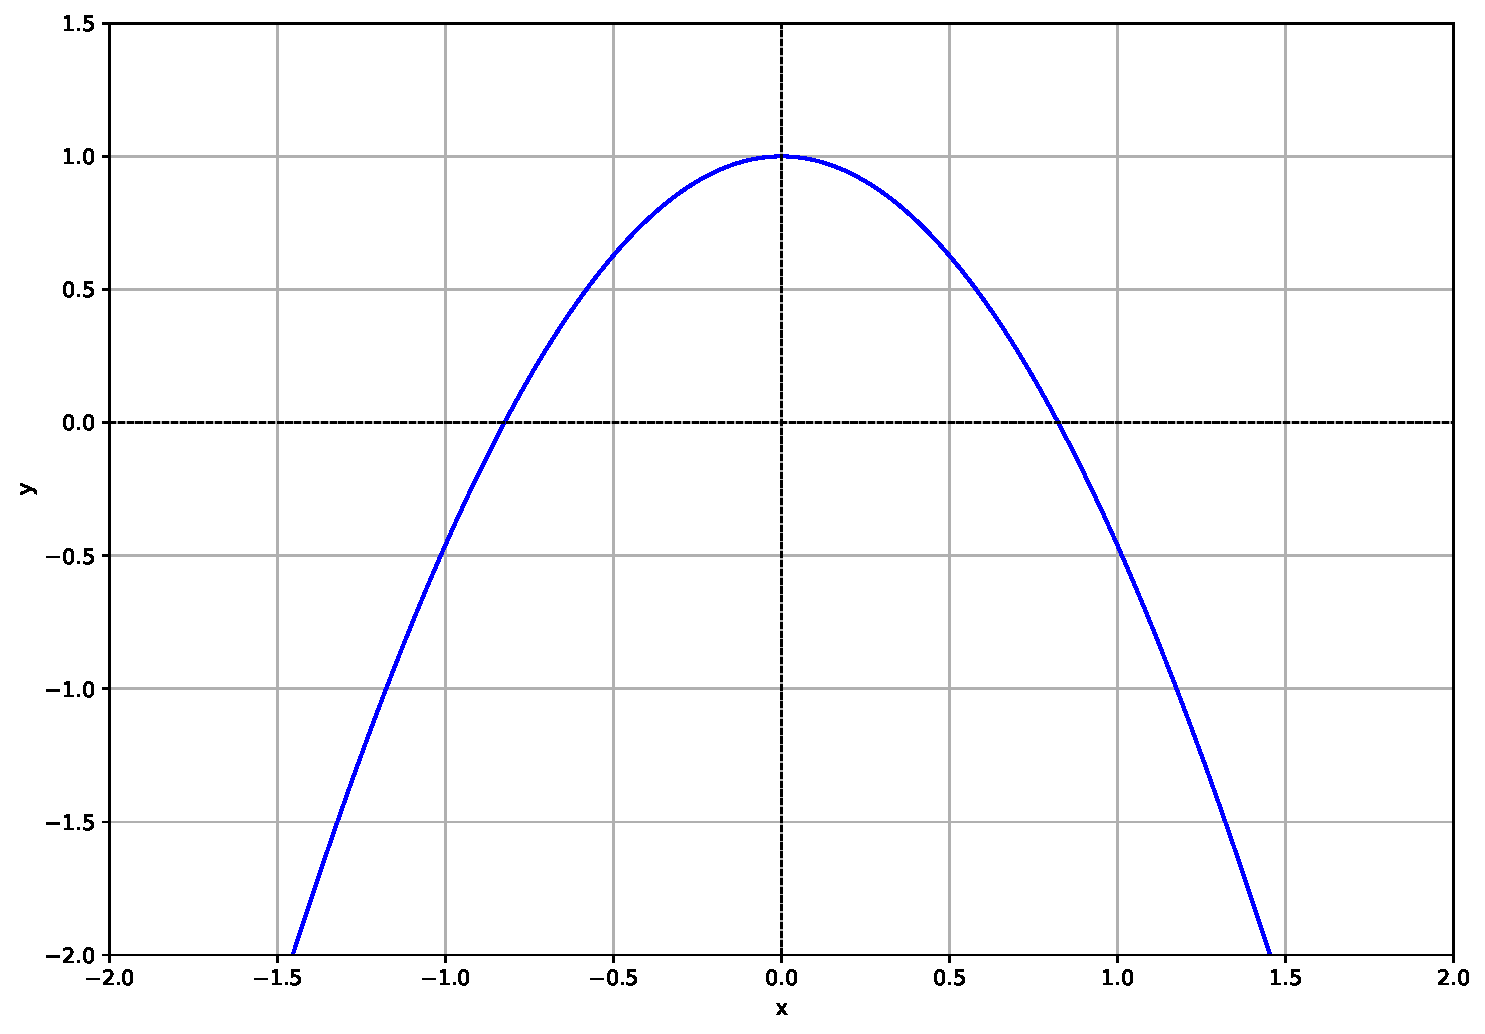
\includegraphics[width=0.9\textwidth]{class_technical_report-main_shiozawaChange/func_graph.pdf}
    \caption{$f(x)=\cos x- x^2$のグラフ}
    \label{fig:func}
\end{figure}


\subsection{2分法・ニュートン法の説明}

まず,二分法についての解説を行う.二分法とは中間値の定理を用いて
方程式の解を求める方法である.中間値の定理とは,関数$y=f(x)$が連続であるとき
x軸上に異なる2点a,b(ただし, a<bとする)
を考えると,f(x)は2点$(a,f(a))$, $(b,f(b))$を通る.
この時,dを$f(a)$と$f(b)$の間の数とすれば,関数は連続であるから,$f(c)=d$
を満たす点cが少なくとも1つaとbの間に存在するというものである.
この中間値の定理を応用し,$f(a)$と$f(b)$が異符号の場合について考る.
まず,区間の中点 $c = (a+b)/2$ を求める.
もし$f(a)$と$f(c)$が異符号,すなわち$f(a)f(c)<0$であれば解は区間$[a,c]$内に存在するため$b$を$c$に更新する.
そうでなければ解は区間$[c,b]$内に存在するため$a$を$c$に更新する.
この操作を反復し,解を含む区間の幅を狭めていくことで解の近似値を得る手法が二分法である.



次にニュートン法についての解説を行う.ニュートン法とは,関数の接線を利用して方程式$f(x)=0$の解を求める数値計算手法である.
まず,解の初期近似値$x_0$を定める.次に,点$(x_0, f(x_0))$における$f(x)$の接線とx軸との交点を求め,これを新たな近似値$x_1$とする.
n番目の近似値$x_n$が与えられたとき,次の近似値$x_{n+1}$は以下の(\ref{eq:newton})式に示される漸化式によって計算される.
\begin{equation}
x_{n+1} = x_n - \frac{f(x_n)}{f'(x_n)}\label{eq:newton}
\end{equation}
この計算を$|x_{n+1} - x_n|$が十分に小さくなるまで反復することで,$f(x)=0$の解の近似値を得る.





\subsection{プログラムの仕様}

まず,二分法により方程式の解を求めるプログラムの解説を行う.
二分法により方程式の解を求める関数として $double\,bisection(double\,a,\,double\,b,\,double\,tol)$
関数を定義した.この関数は引数としてaの座標,$b$の座標,許容誤差をもつ.区分が間違っていたら-1を返し,
区分があっていたら$a$と$b$の中点$c$を求め,もし$c$の値が負の数なら$b$の値を$c$とし,そうでなければ$a$の値を$c$とする
ことで,$a$と$c$の距離を許容誤差$tol$を下回るまで狭めていく.このループ中にコンソールとcsv形式の
ファイルにループ毎にループ回数と
ループ毎の$a$と$c$の距離を出力し,解が収束したら$c$の値を返す関数になっている.
この関数を使用することで何回のループ処理で解を求めることができたかと,どのような
過程で値が収束していったかと解の値を調べる.

次にニュートン法により方程式の解を求めるプログラムの解説を行う.
ニュートン法により方程式の解を求める関数として $double\,newton(double\,x0,\,double\,tol,\,int\,max\_iter)$
関数を定義した.この関数は引数として初期の近似解$x0$と許容誤差$tol$と最大ループ回数$max\_iter$をもつ.
まず最初に$f(x_n) / df(x_n)$によって得られる値を求めそのループ時の近似解$x_n$と$f(x_n)$における接線とx軸との交点
の距離$h$を求める.そして$x_n$から$h$の値を引くことで次の近似解
$x_{n+1}$を求める.この処理を$h$の値が許容誤差$tol$よりも小さくなり収束したと判断されるかループ回数が
最大ループ回数$max\_iter$を上回り解が収束しないと判断されるまで繰り返す.
このループ中にコンソールとcsv形式の
ファイルにループ回数とループ毎の$h$の値を出力し,解が収束したらその時の近似解の値を返す関数になっている.
この関数を使用することで何回のループ処理で解を求めることができたかと,どのような
過程で値が収束していったかと解の値を調べる.


\subsection{評価指標}
今回は解を求めるまでの処理のループ回数が少ないかと
解の誤差をより速く縮められているかを
速く解を求められるということの評価指標とする.

\section{結果}
プログラムを実行した結果得られた二分法とニュートン法の推定解が収束していく様子
と繰り返し回数あたりの誤差を図\ref{fig:kekka}に示す.



\begin{figure}[H]
    \centering
    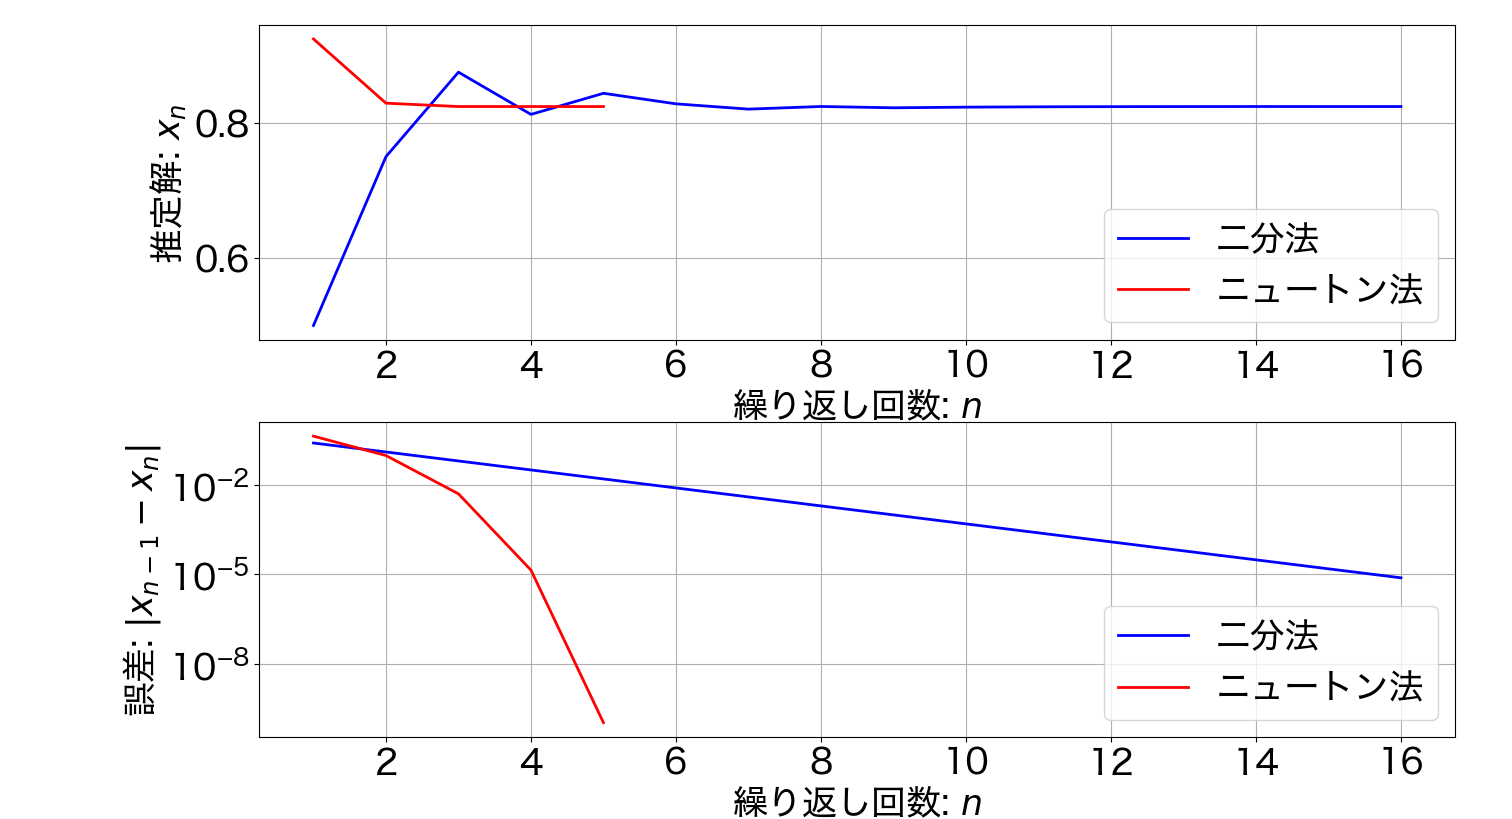
\includegraphics[width=0.9\textwidth]{class_technical_report-main_shiozawaChange/Figure_kekka.png}
    \caption{上図:推定解が収束していく様子/下図:繰り返し回数あたりの誤差}
    \label{fig:kekka}
\end{figure}

結果,解はどちらも約$0.824$に収束し,二分法の解が収束するまでのループ回数は16回で,誤差は最終的に
$10^{-5}$になることと,ニュートン法の解が収束するまでのループ
回数は5回で,誤差は最終的に$10^{-10}$になることが分かった.

\section{おわりに}

\subsection{まとめ}
今回は二分法とニュートン法のどちらのほうが方程式の解をより
速く求める事ができるか調査した.
二分法とニュートン法それぞれの方法を使って
解を求めるプログラムを制作し,
それぞれ値が収束するまでに何回反復計算を行ったか調べた.
結果,二分法は16回,ニュートン法は5回繰り返し計算を行っていることがわかった.

\subsection{考察}

まず,二分法とニュートン法のどちらが方程式の解をより速く求められるかの考察を行う.
評価指標にある解を求めるのにかかったループ回数に関してはニュートン法はループ回数が5回,
二分法はループ回数が16回であることからニュートン法のほうが速く解を導けると考えることができる.
また,もう一つの評価指標である解の誤差をより速く縮められているかという点についても
誤差が$10^{-5}$になるまでニュートン法はループ回数が4回,二分法はループ回数が16回であることから
やはりニュートン法のほうが速く解を求められるということが分かる.
この結果は早稲田大学の— 非線形方程式の解法 (1) —\cite{waseda}という資料にある二分法より高速に解に収束することが多い
という記述と一致するため,結果は妥当であると考えられる.

次に,計算回数が指定されていた場合どちらのほうが解に近づくことができるかについての考察を行う.
図\ref{fig:kekka}の下図から誤差が小さくなる様子の比較を行うと
二分法はほぼ一定の間隔で緩やかに誤差が小さくなっているがニュートン法は二回目以降誤差が
急激に小さくなる事がわかる.このことから計算の回数が指定されている場合であっても
二回以上の試行回数が与えられるならニュートン法のほうが速く解に近づくことができる
という事が考えられる.

今後の調査の課題についての考察を行う.今回は計算の反復回数を評価指標としたが,一回の反復で行われる計算の回数は考慮していない.
二分法は一回のループで行う処理がa点とb点の中間を求め,その中間の値が正か負かで値を更新するというシンプルなもの
だが,ニュートン法は$f(x_n) / df(x_n)$によってそのループ時の近似解$x_n$と$f(x_n)$における接線とx軸との交点
の距離$h$を求め,$x_n$から$h$の値を引くことで次の近似解$x_{n+1}$を求める処理が必要であり,
二分法に比べて一回のループで行う処理の回数が多い.そのためニュートン法のほうが少ない
ループ回数で解を求められるとしても全体の処理時間に関しては確実にニュートン法のほうが
速く処理が終わっているかについての検証を行えていないということが今回の手法の問題点であると考えられる.
また,今回は(\ref{eq:fx})式を用いての検証しか行っていないため,他の関数の場合でも
同様にニュートン法の方が速く解が収束するかの検証も行えていないため,この点についても
今後検証を行う必要があると考えられる.

\subsection{結論}
今回行った調査の結果,ニュートン法の方が少ないループ回数で
非線形方程式の解を求められるということが分かった.
そのため非線形方程式の解を速く求めたい時はニュートン法を用いた方が良いと言える.
しかし,今回の調査ではあくまでも計算のループ回数の検証しか行えていなく,
実際に計算にかかる時間については考慮していないため,今後の検証では
ループ回数だけでなく1回のループにかかる時間や他の関数で検証しても同様の事が言えるかについての
検証も行い,確実にニュートン法のほうが速く解を求められるか検証する必要がある.

\begin{thebibliography}{5}

\bibitem{omu} 近畿大学, オームの法則,
2025年7月2日閲覧, \url{https://www.phys.kindai.ac.jp/laboratory/kondo/lectures/ichikawa/ELE2p19-34.pdf}

\bibitem{toutyo} 兵庫県立大学, 速さ (等速直線運動,変位),
2025年7月2日閲覧, \url{https://www.eng.u-hyogo.ac.jp/msc/msc12/HIT/html/rikigaku/pdf/Chapter-1.pdf}


\bibitem{daio} 広島大学, 非線形素子 ~~ 固体の電子を制御せよ ~~, 
2025年7月2日閲覧, \url{https://home.hiroshima-u.ac.jp/ino/lecture/SSP1slide12_ino2017.pdf}


\bibitem{jinko} 九州産業大学, ロジスティック曲線, 
2025年7月2日閲覧, \url{https://design.kyusan-u.ac.jp/OpenSquareJP/?LogisticCurve}


\bibitem{waseda} 早稲田大学, — 非線形方程式の解法 (1) —, 
2025年7月2日閲覧, \url{https://yuuka.w.waseda.jp/cpro2/Cpro2_10th.pdf}

\end{thebibliography}
\end{document}



























